\chapter{Méthodes de travail}

% Méthodes de travail
% Organisation temporelle, spatiale, humaine 
% interactions des membres de l’équipe projet
% interactions avec les encadrants
% interactions avec les tiers

\section{Communication}
\vspace{1.5cm}
Tout au long du projet notre méthode de travail a changée. Au fur et à mesure que les séances s’enchaînaient, et en prenant en compte les conseils qui nous ont été donnés (notamment à propos du carnet de bord et des objectifs à court terme) notre méthode de travail a tendu vers la suivante : \\ \\
De manière générale, toute l'équipe du projet BMONS travaille dans la même salle pour faciliter la communication entre les membres du groupe. Une séance de travail commence par l'ouverture personnelle des mails de chacun, puis le groupe se réunit pour définir les objectifs de la matinée, ensuite chacun choisit la partie il va avancer. Le travail se fait en général seul ou en binôme et des points d'avancement sont faits à l'oral tout au long de la séance. Parfois des tâches comme la prise en main d'un logiciel ou la compréhension d'un diagramme sont faites en dehors des séances, mais la majeure partie du travail s'effectue lors du temps alloué au projet. \\ \\
Les réunions avec les encadrants et les intervenants extérieurs se déroulent dans des salles de l'ENSTA Bretagne équipées d'un vidéo projecteur et en présence de la totalité de l'équipe BMONS. Ces séances sont organisées à l'avance, les points sur lesquels des précisions sont nécessaires sont mis en avant avant la séance et des questions précises sont préparées. Cela permet de guider la réunion et de ne pas perdre de temps sur des points déjà vus. Chacun a son rôle lors de ces réunions, la prise de notes, le dialogue avec l'intervenant et la rédaction du compte rendu sont ainsi facilités.

\section{Outils pour les échanges}
\vspace{1.5cm}
% Quels sont les outils qui nous permettent de travailler ensemble ?

Les outils qui nous ont permis de travailler ensemble et de partager nos fichiers ont également changés au cours du temps. 
Avant les premiers ateliers techniques, particulièrement celui sur github, nous partagions nos résultats sur le oneDrive d'office 365. Cet outil est efficace pour partager des documents, mais n'est pas optimisé pour le travail simultané de plusieurs membre du groupe sur un même document. \\
Nous avons donc utilisé github (figure \ref{fig:InterfaceGit}), malgré une prise en main un peu longue pour ceux d'entre nous qui n'ont pas assisté a l'atelier, github s'est révélé être un outil optimisé pour le travail que nous faisons. Le journal de bord, et les objectifs à cours termes en particulier, sont regroupé dans un wiki (figure \ref{fig:ExempleWiki}) que chacun peu consulter, les liens utiles au projet y sont également répertoriés. Notre projet étant open source, la totalité de ces informations sont accessible par tous ceux qui souhaitent s'informer sur l'avancement du projet, ainsi nous avons reçus un mail de la part d'une de ces personnes nous invitant à suivre un projet similaire.

\begin{figure}[h!]
\centering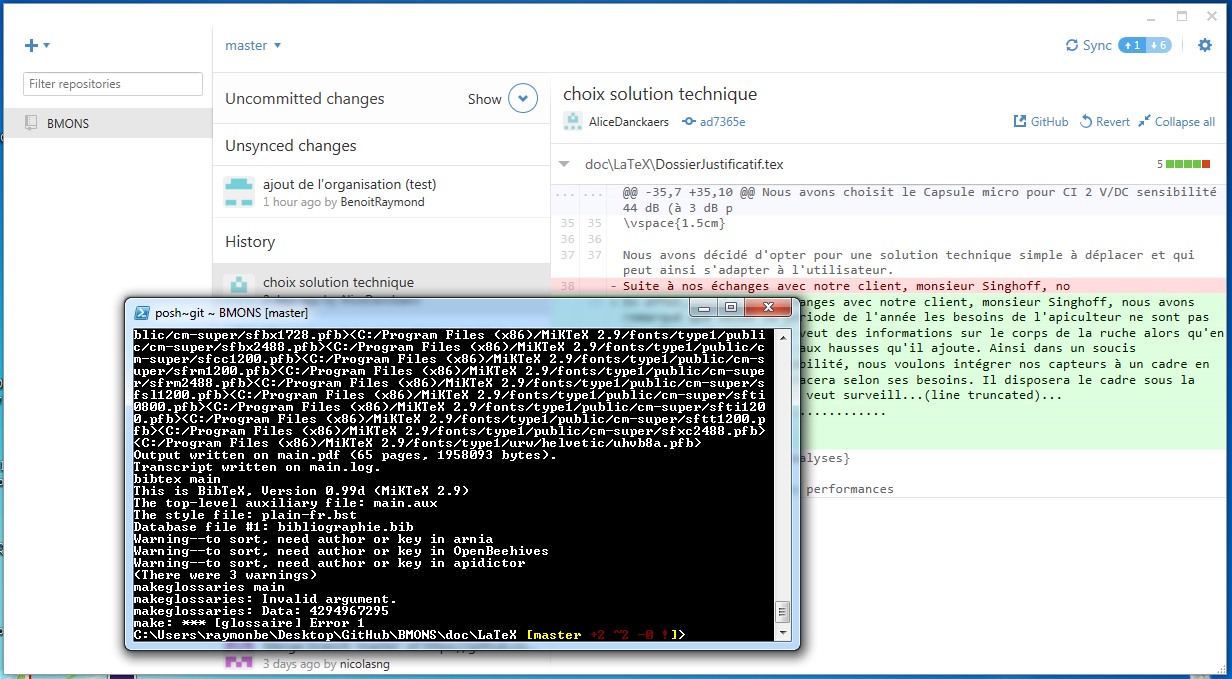
\includegraphics[scale=0.5]{InterfaceGit.png}
\caption{\label{fig:InterfaceGit} interface de travail gitHub}
\end{figure}

\begin{figure}[h!]
\centering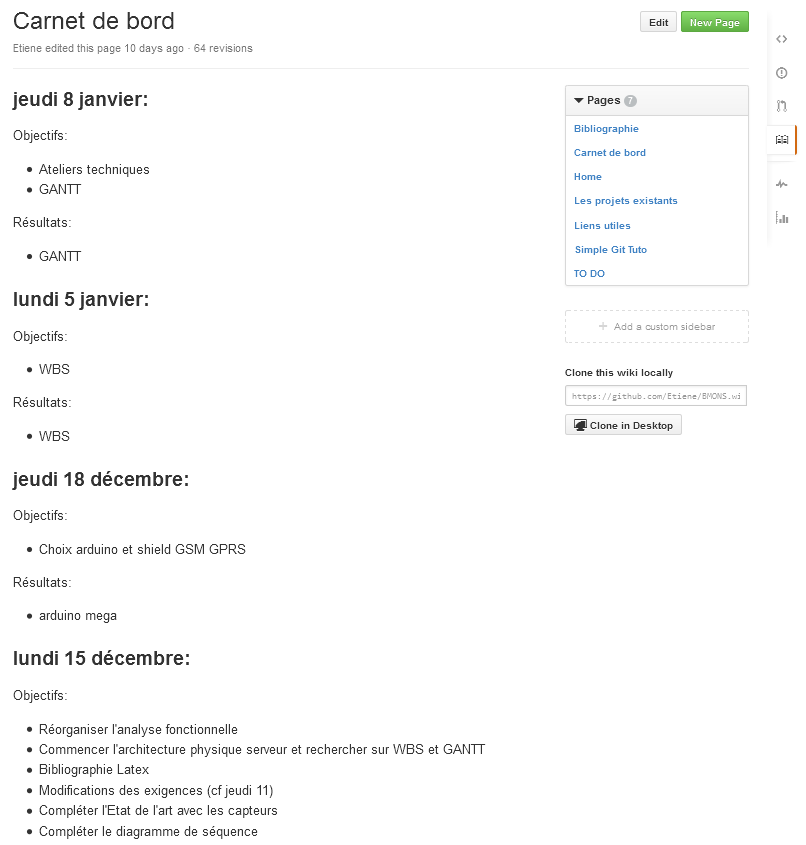
\includegraphics[scale=0.55]{ExempleCarnetDeBord.png}
\caption{\label{fig:ExempleWiki} Exemple d'utilisation du wiki de gitHub}
\end{figure}

\chapter{Répartition des tâches}

\section{Structure de découpage du projet}
\vspace{1.0cm}
Structure de découpage du projet, ou Work Breakdown Structure (WBS) en anglais, est un diagramme hiérarchique, axée sur les tâches et activités que l’équipe de projet doit exécuter pour atteindre les objectifs du projet.

Dans cette partie nous allons analyser nos tâches. Elles sont divisés en deux parties: Serveur et Arduino. La partie serveur comprend tout ce qui est lié au développement du site ainsi que les scripts qui contrôlent les logiciels, les backups et l'obtention de données. La partie arduino comprend tous les capteurs et modules, l'énergie et les scripts de contrôle des capteurs et manipulation des données.  
\begin{figure}[h!]
\centering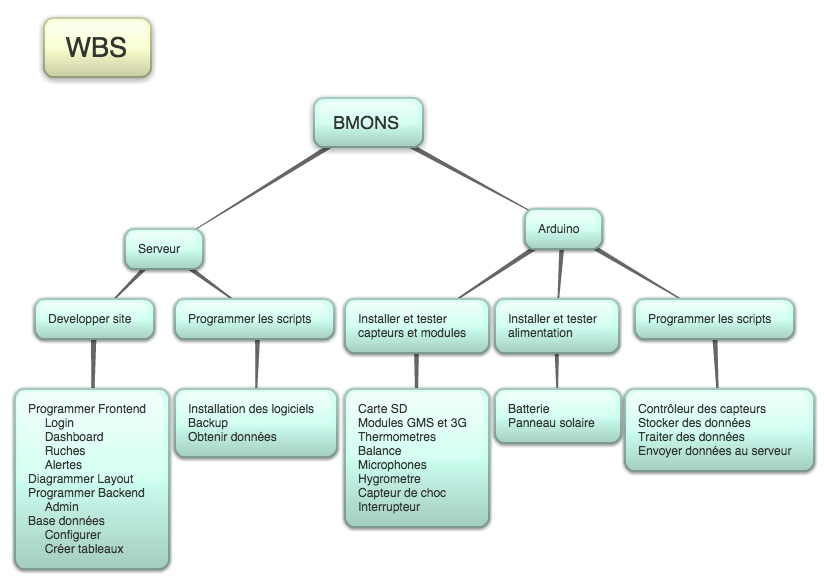
\includegraphics[scale=0.40]{WBS2.png}
\caption{\label{fig:SDP} Structure de découpage du projet du système BMONS}
\end{figure}

\clearpage

\section{Diagramme de Gantt}
\vspace{1.5cm}
Le diagramme de Gantt est un outil utilisé en gestion de projet permettant de visualiser dans le temps les diverses tâches composant un projet. Il s'agit d'une représentation qui permet de représenter graphiquement l'avancement du projet par les séances. Les tâches du projet BMONS sont divisés en deux catégories, Serveur et Arduino, comme dans le structure de découpage du projet, en permettant que l'équipe se sépare en deux et partage les tâches en travaillant de façon concomitante.
\vspace{1.5cm}
\begin{figure}[h!]
\centering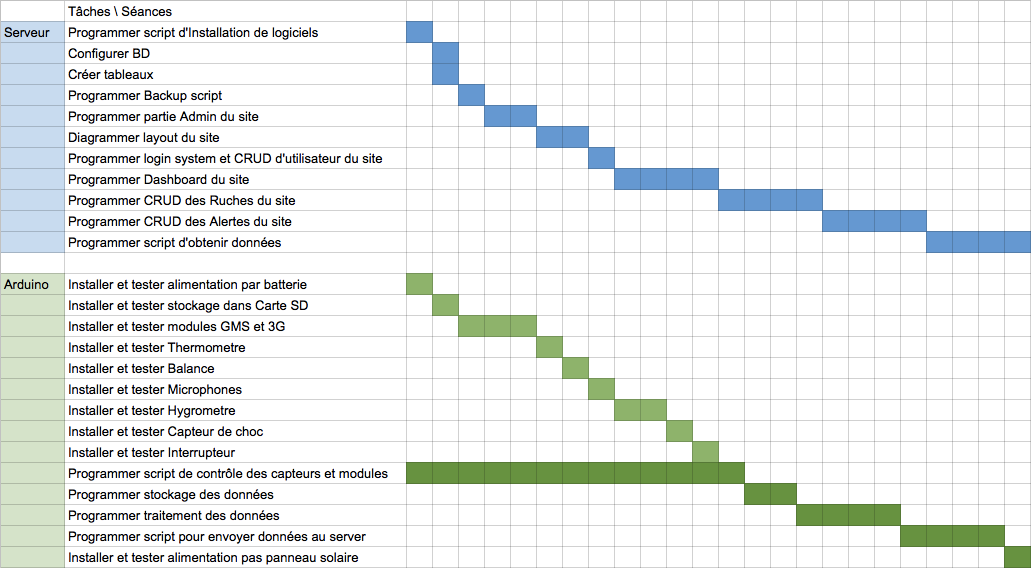
\includegraphics[scale=0.45]{GANTT2.png}
\caption{\label{fig:GANTT} Diagramme de Gantt du système BMONS}
\end{figure}


% WBS et diagramme de Gantt
